\documentclass[tikz,border=10pt]{standalone}
\usetikzlibrary{calc}

\begin{document}
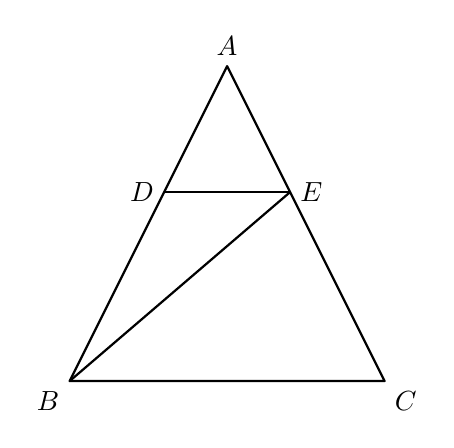
\begin{tikzpicture}[scale=2, thick, line join=round]
    % 1. 定义顶点坐标
    % 使用相对位置设定 A, B, C，使三角形比例协调
    \coordinate (B) at (0,0);
    \coordinate (C) at (2,0);
    \coordinate (A) at (1,2);
    
    % 2. 定义 D 和 E 点（假设 DE 平行于 BC，取边长的 1/2）
    \coordinate (D) at ($(A)!0.4!(B)$);
    \coordinate (E) at ($(A)!0.4!(C)$);
    
    % 3. 绘制三角形主体
    \draw (A) -- (B) -- (C) -- cycle;
    
    % 4. 绘制内部线段
    \draw (D) -- (E); % 平行线
    \draw (B) -- (E); % 斜线
    
    % 5. 标注点位
    \node[above] at (A) {$A$};
    \node[below left] at (B) {$B$};
    \node[below right] at (C) {$C$};
    \node[left] at (D) {$D$};
    \node[right] at (E) {$E$};

\end{tikzpicture}
\end{document}